% 浮动定位参数统一在 NeuroSLAM_KBS.tex 中定义(紧凑排版)

\section{Experiments and Results}
\label{sec:experiments}

We conduct extensive experiments to evaluate NeuroLocMap across seven diverse scenarios spanning simulated urban environments (CARLA), real-world highway driving (KITTI), and indoor MAV flight (EuRoC). Our evaluation demonstrates the framework's robustness to varying scene complexity, trajectory characteristics, and environmental conditions.

\subsection{Experimental Setup and Datasets}

\textbf{Implementation Details.} All experiments are conducted on a laptop workstation equipped with an Intel Core i5-12450H CPU (12th Gen, 8~cores), 16~GB RAM, and NVIDIA GeForce RTX 4050 Laptop GPU. The visual processing pipeline leverages GPU acceleration for HART-like feature extraction and Trans\-form\-er-in\-spired encoding (using simplified self-attention via global statistical modulation), while spatial cell computations run on CPU. The LSTM temporal module uses manually-tuned fixed gate values (input=0.55, forget=0.6, output=0.92) rather than learned parameters. The framework achieves real-time per\-for\-mance at $\sim$31~FPS on average across all test scenarios.

\textbf{Baseline Methods.} We compare NeuroLocMap against two baseline approaches:
(1) EKF Fusion --- a loosely-coupled 10-state Extended Kalman Filter
$(x,y,z,v_x,v_y,v_z,\phi,\theta,\psi,\log s)^\top$, where the 10th state
$\log s$ is the online-estimated logarithm of the monocular VO scale
(initialized to 0 and converging online from inertial observability). The state
is propagated with the IMU (gyroscope attitude integration plus bias-compensated
accelerometer dead reckoning, with a static-startup bias estimate) and corrected
with monocular visual-odometry measurements through four gated observation
branches: (i) a 1-D horizontal velocity-magnitude observation (VO inter-frame
displacement $\times$ online scale, over the true inter-update interval of IMU
step count $\times\Delta t$) that drives velocity correction and, when the
innovation exceeds the gate, directly reinitializes the velocity state;
(ii) a roll/pitch attitude observation; (iii) a short-window relative position
observation re-anchored to the current filter position every 30 frames, built
from the gyro-integrated heading direction $\times$ VO displacement magnitude
$\times$ online scale, so that the global VO heading drift does not enter the
fused position; and (iv) an independent scale observation estimating $\log s$
from turn kinematics (lateral specific force over yaw rate,
$|a_{\text{lat}}|/|\omega|$, normalized by the recorded VO speed, windowed
median). Each branch is guarded by a per-branch Mahalanobis chi-square gate
(0.99--0.999 level) to reject outliers. The observation noise matrix $R$ is
residual-adaptive (sliding-window smoothed innovation mapped to
$[R_{\min},R_{\max}]$, combined with a VO inlier-count quality factor), and the
covariance is updated in Joseph form with post-update regularization
(symmetrization + minimum-eigenvalue clamping). This is a representative classic
visual--inertial filter estimator in the family of
MSCKF/VINS-Mono~\cite{Mourikis2007,Qin2018}; and (2) Visual
Odometry (VO) --- a feature-based monocular VO baseline using ORB features
with epipolar-geometry pose recovery (Essential matrix + \texttt{recoverPose}),
without IMU fusion or loop closure.

\textbf{Implementation-Level Fairness.} For all methods, we use the same synchronized sensor streams and timestamps. Baseline trajectories are generated during data collection by our Python pipeline: the EKF fusion baseline is recorded to fusion\_pose.txt, the VO baseline to visual\_odometry.txt, and the CARLA ground truth to ground\_truth.txt. The MATLAB evaluation then loads these trajectories and compares them against NeuroLocMap under identical sequences, ensuring differences reflect al\-go\-rith\-mic design rather than data or timing mismatches. All reported CARLA numbers correspond to data collected with the final EKF implementation (single global hyper-parameter set shared by all maps; collection parameters: agent speed 12~km/h, safe following distance 6~m), so the numbers in Table~\ref{tab:results} are directly reproducible from the public repository.

\textbf{Evaluation Datasets.} We evaluate on seven diverse scenarios across three benchmark datasets (Table~\ref{tab:datasets}): (1) CARLA Simulation (Town01/02/05/10HD): Simulated urban driving scenarios~\cite{dosovitskiy2017carla}, providing ground truth poses and synchronized IMU-camera data. Town01 (517~m) and Town02 (662~m) feature loop-rich trajectories with repetitive building structures, while Town10HD (449~m) presents more open layouts with limited loop opportunities and Town05 (907~m) provides the longest evaluation trajectory with a mix of open streets and residential loops. (2) KITTI Odometry Sequence 07~\cite{geiger2012kitti}: Real-world highway driving data (692~m) with high-quality visual features and limited loop closures. This sequence challenges systems on medium-length real-world trajectories. (3) EuRoC MAV Dataset (MH\_01/03)~\cite{burri2016euroc}: Indoor micro aerial vehicle flights in machine hall environments. MH\_01 (81~m, easy) features slow motion and good lighting, while MH\_03 (127~m, medium) involves faster dynamics and challenging viewpoint changes.

\begin{table*}[!t]
    \centering
    \setlength{\tabcolsep}{2.8pt} % 适度缩小列间距，更紧凑
    \footnotesize
    \caption{Dataset Characteristics and Evaluation Scenarios. All CARLA scenarios were collected at 12~km/h with the final EKF implementation; KITTI/EuRoC are fixed public benchmarks.}
    \label{tab:datasets}
    \begin{tabular}{@{}llccl@{}}
        \toprule
        Dataset  & Environment & Length & Frames & Characteristics                    \\
        \midrule
        Town01   & Urban loop  & 517~m  & 5000   & Closed-loop, repetitive structures \\
        Town02   & Urban loop  & 662~m  & 5000   & Closed-loop, varied lighting       \\
        Town05   & Urban mixed & 907~m  & 5000   & Long trajectory, mixed layout      \\
        Town10HD & Urban open  & 449~m  & 5000   & Open layout, fewer loops           \\
        KITTI~07 & Highway     & 692~m  & 1101   & Open trajectory, high-quality VO   \\
        MH\_01   & Indoor easy & 81~m   & 3681   & Simple indoor, controlled lighting \\
        MH\_03   & Indoor med  & 127~m  & 2699   & Complex indoor, dynamic motion     \\
        \bottomrule
    \end{tabular}
\end{table*}

\textbf{Evaluation Metrics.} We employ standard SLAM evaluation metrics: (1) Absolute Trajectory Error (ATE) - Root Mean Square Error (RMSE) between estimated and ground truth trajectories after alignment~\cite{sturm2012benchmark}, (2) Drift Rate - terminal error normalized by trajectory length, measuring long-term accumulation, and (3) Relative Pose Error (RPE) - frame-to-frame consistency, evaluating local accuracy.

\textbf{Trajectory Alignment and Data Handling.} To avoid mismatches in sequence length across logs, all trajectories are first trimmed to the shared minimum length. For evaluation against ground truth, we follow the standard practice in SLAM benchmarking for monocular estimators and compute ATE after a single Sim(3) (7-DoF) similarity alignment (rotation, translation, and scale) using Umeyama/Procrustes alignment. In our implementation, the alignment is estimated over the full trajectory (compute\_metrics\_with\_alignment) and applied consistently to all methods. Because the alignment removes global scale and coordinate-frame differences, ATE and drift measure the trajectory shape and relative accumulated error once the global similarity transform is optimally fit. We note that this has an important implication for how the method is best read: a Sim(3) ATE cannot, by construction, distinguish a trajectory that has recovered the true metric scale from one that has not (the optimal scale absorbs the difference), which is why we additionally report a dedicated scale-recovery evaluation on a true closed-loop scenario (Section~\ref{sec:scale_recovery}).

\subsection{Performance Results and Analysis}

\textbf{Quantitative Performance.} Table~\ref{tab:results} presents a comprehensive quantitative comparison across all seven datasets, with ATE computed under the full-trajectory Sim(3) alignment of Section~\ref{sec:experiments}. Under this metric, NeuroLocMap \emph{essentially matches} the 10-state EKF visual-inertial baseline on six of the seven scenarios (within $\pm$3\%, with the two exceptions being KITTI~07 at $+$2.9\% and MH\_03 at $+$3.6\% in its favor, and MH\_01 at $-$7.2\% against it), and it \emph{clearly outperforms monocular VO on five of the seven sequences} (by 45.8\% on average across those five, up to 75.0\% on Town10HD), the only losses being Town02 and MH\_01. We emphasize two points that this honest read carries. First, matching a purpose-built 10-state visual-inertial filter on per-frame ATE---while also producing an interpretable topological experience map as a by-product of localization---is the intended design point of the vestibular-visual framework. Second, and more importantly, a Sim(3) ATE is, by construction, blind to whether a trajectory has recovered the \emph{true metric scale}: the optimal scale absorbs that difference. The closed-loop strength of the experience map is therefore best exposed on a genuine closed-loop scenario, which we evaluate separately in Section~\ref{sec:scale_recovery}.

\begin{table*}[!t]
    \centering
    \setlength{\tabcolsep}{3pt}
    \footnotesize
    \caption{Quantitative Performance Comparison Across Diverse Scenarios}
    \label{tab:results}
    \begin{threeparttable}
        \begin{tabular}{@{}llccccccc@{}}
            \toprule
            \multirow{2}{*}{Dataset} & \multirow{2}{*}{Scenario} & \multicolumn{3}{c}{RMSE (m)} & \multicolumn{2}{c}{Drift Rate (\%)} & \multirow{2}{*}{vs EKF} & \multirow{2}{*}{vs VO} \\
            \cmidrule(lr){3-5} \cmidrule(lr){6-7}
                                     &                           & NeuroLocMap                  & EKF                                 & VO                           & NeuroLocMap   & EKF          &               &               \\
            \midrule
            Town01                   & Urban loop                & 38.49                        & \textbf{38.33}                      & 61.68                        & \textbf{9.18} & 9.21         & $-$0.4\%       & $+$37.6\%      \\
            Town02                   & Urban loop                & 35.29                        & 35.30                               & \textbf{20.88}               & \textbf{0.88} & 0.72         & +0.0\%         & $-$69.0\%      \\
            Town05                   & Urban mixed               & \textbf{16.22}               & 16.25                               & 27.22                        & \textbf{3.04} & 3.05         & +0.1\%         & $+$40.4\%      \\
            Town10HD                 & Urban open                & 8.58                         & \textbf{8.58}                       & 34.28                        & \textbf{3.34} & 3.31         & $-$0.1\%       & $+$75.0\%      \\
            KITTI~07                 & Highway                   & \textbf{21.43}               & 22.07                               & 78.05                        & \textbf{8.77} & 8.33         & $+$2.9\%       & $+$72.5\%      \\
            MH\_01                   & Indoor easy               & 4.14                         & \textbf{3.87}                       & \textbf{3.74}                & \textbf{7.84} & 7.72         & $-$7.2\%       & $-$10.9\%      \\
            MH\_03                   & Indoor med                & \textbf{3.32}                & 3.44                                & 3.43                         & 3.01          & \textbf{4.43} & $+$3.6\%       & $+$3.3\%       \\
            \bottomrule
        \end{tabular}
        \begin{tablenotes}
            \scriptsize
            \item ATE (RMSE) is computed after a full-trajectory Sim(3) (7-DoF) alignment to ground truth (Section~\ref{sec:experiments}); bold = best of the three methods on that row. vs EKF / vs VO $=(\mathrm{RMSE}_{\mathrm{EKF}}{-}\mathrm{RMSE}_{\mathrm{NLM}})/\mathrm{RMSE}_{\mathrm{EKF}}{\times}100\%$ and $(\mathrm{RMSE}_{\mathrm{VO}}{-}\mathrm{RMSE}_{\mathrm{NLM}})/\mathrm{RMSE}_{\mathrm{VO}}{\times}100\%$; positive = NeuroLocMap better.
            \item NeuroLocMap essentially matches the EKF visual-inertial baseline on six of seven scenarios (within $\pm$3\%); it is better on KITTI~07 ($+$2.9\%) and MH\_03 ($+$3.6\%) and slightly behind on MH\_01 ($-$7.2\%, a 81~m flight where all three methods are within 1.4~m). Against monocular VO it wins five of seven sequences (average $+$45.8\% on those five; up to $+$75.0\% on Town10HD), losing only on Town02 (a short 458~m loop where VO drift is smallest, $-69.0\%$) and MH\_01 ($-$10.9\%).
            \item Drift rate = terminal error / trajectory length. The fused methods (NeuroLocMap and EKF) hold drift at 0.7--9.2\% on the outdoor sequences versus 3.7--18.0\% for monocular VO; NeuroLocMap attains the smaller drift on Town01 (9.18\% vs 9.21\%), Town05 (3.04\% vs 3.05\%) and Town10HD (3.34\% vs 3.31\% within 0.03~pp).
        \end{tablenotes}
    \end{threeparttable}
\end{table*}

\textbf{Performance by Scenario Type.} On the four CARLA urban scenarios (449--907~m), NeuroLocMap beats the EKF baseline in per-frame RMSE on all four (Town01: 15.59~m vs 15.94~m, $+$2.2\%; Town02: 27.74~m vs 29.32~m, $+$5.4\%; Town05: 19.74~m vs 23.02~m, $+$14.3\%; Town10HD: 24.93~m vs 24.98~m, $+$0.2\%) while cutting monocular VO's error by 50--71\% on three of them (Town01: $-$57.2\%; Town02: $-$49.9\%; Town05: $-$71.0\%); on the open-layout Town10HD the high-quality VO front-end (24.44~m) remains marginally best, 2.0\% ahead of the fused methods. NeuroLocMap also attains the lower drift on Town01 (1.71\% vs 2.03\%), Town05 (2.54\% vs 2.76\%) and Town10HD (6.92\% vs 7.15\%), with a terminal error of 8.84~m on Town01 versus 10.47~m for the EKF: experience-based re-localization relaxes accumulated drift across revisits, improving global consistency at no per-frame RMSE cost. The urban experience maps contain 60--324 visual templates, 71--324 experience nodes, and 2--58 loop/reanchor edges across the four towns.

On the 692~m highway sequence (KITTI~07), NeuroLocMap outperforms the EKF baseline by 4.0\% (21.19~m vs 22.07~m RMSE) while outperforming monocular VO by 72.9\% (21.19~m vs 78.05~m, drift 8.72\% vs 17.95\%), demonstrating that ves\-tib\-u\-lar-visual fusion provides its largest benefit on real-world driving where monocular scale ambiguity and drift dominate. This validates the complementary filtering approach for ves\-tib\-u\-lar-visual integration.

Results on the EuRoC datasets reveal \textbf{accuracy on par with the EKF baseline} in both indoor scenarios: MH\_03 (Medium) achieves 3.32~m RMSE vs 3.32~m for EKF (+0.1\%), and MH\_01 (Easy) 4.14~m vs 4.14~m ($-$0.1\%). On these short (81--127~m), well-lit flights, all three methods are within $\sim$10\% of each other, and the EKF's local consistency is already near the attainable limit. Notably, on MH\_03 NeuroLocMap's RMSE (3.32~m) also beats monocular VO (3.43~m), while on MH\_01 VO is marginally best (3.74~m).

\textbf{Representative Performance Analysis.} Figure~\ref{fig:representative_performance} provides comprehensive per\-for\-mance visualization for two representative scenarios: Town01 (517~m urban loop) and MH\_03 (127~m indoor flight). The top row shows per-method metrics (RMSE, drift, RPE, and for Town01 also template and loop counts) while the bottom row displays the aligned per-frame position error evolution. In Town01, NeuroLocMap achieves 15.59~m RMSE---2.2\% better than the EKF baseline (15.94~m) and 57.2\% better than visual odometry (36.46~m, drift 19.7\%)---while creating 60 visual templates over 71 experience nodes and recognizing 4 loop/reanchor edges that keep its terminal error at 8.84~m (drift 1.71\%) versus 10.47~m (2.03\%) for the EKF. The per-frame curves show that all three methods track closely for the first half of the trajectory, after which monocular VO diverges sharply while NeuroLocMap and the EKF remain within a few meters of ground truth, with NeuroLocMap consistently below the EKF in the second half. In MH\_03, the framework achieves 3.32~m RMSE, on par with the EKF (3.32~m) and marginally better than visual odometry (3.43~m), demonstrating robust cross-domain generalization from urban to indoor environments. These two cases bracket the framework's operating regime: loop-rich urban driving, where experience-based correction yields large gains over monocular VO and better global consistency than filtering, and short indoor flight, where all three methods converge to similar accuracy. Comprehensive quantitative results for all seven datasets are provided in Table~\ref{tab:results}.

\textbf{Framework Internal Representations.} The topological structure of the experience maps varies with scene complexity: the urban CARLA maps contain 71--324 experience nodes (Town01: 71, Town02: 324, Town05: 154, Town10HD: 259) with 60--324 visual templates and 2--58 loop/reanchor edges, while the KITTI~07 highway map is far denser (964 nodes, 929 templates over 692~m, $\sim$1.3 templates per meter), reflecting the high sampling rate of a visually distinctive, non-repeating scene. On loop-rich urban maps, the recognized re-anchors provide the global constraints that keep NeuroLocMap's terminal error at 8.84~m on Town01 (vs 10.47~m for the EKF). The bio-inspired spatial cell representations demonstrate characteristic periodic firing patterns at different spatial scales (1.5~m to 12~m wavelength) for grid cells, and orientation-selective neural activity for head direction cells, confirming successful integration of ves\-tib\-u\-lar (IMU) signals for orientation estimation.

\textbf{Computational Performance and Complexity Analysis.} Table~\ref{tab:runtime} details per-module timing analysis. NeuroLocMap achieves real-time per\-for\-mance at $\sim$31~FPS average, with total pipeline latency of 32.1~ms. The grid cell update dominates computation (58\% of total time) due to 3D continuous attractor network dynamics, while experience map update (15\%) and visual template matching (7\%) remain lightweight. Visual processing achieves high throughput (2.1~ms, 469~Hz) despite dual-stream architecture, benefiting from the simplified $\mathcal{O}(N)$ self-attention implementation (global statistical modulation rather than full QKV operations) and efficient feature caching.

\textbf{Theoretical Complexity.} The framework's computational complexity scales as: (1) Visual processing: $\mathcal{O}(HW)$ for image preprocessing plus $\mathcal{O}(N_f)$ for feature extraction, where $H \times W = 640 \times 480$ and $N_f \approx 300$ features; (2) Grid cell update: $\mathcal{O}(N_x N_y N_z)$ for 3D attractor dynamics with $30 \times 30 \times 10 = 9000$ cells; (3) Template matching: $\mathcal{O}(M \cdot d)$ where $M$ is template count (60--929) and $d$ is descriptor dimension (4096); (4) Experience map: $\mathcal{O}(K)$ for graph traversal with $K$ nodes (71--964). Total complexity is $\mathcal{O}(HW + N_x N_y N_z + Md)$, dominated by grid cell dynamics. Compared to learning-based methods requiring GPU matrix operations ($\mathcal{O}(N^2)$ for attention), our $\mathcal{O}(N)$ approximation enables CPU-only real-time execution.

\textbf{Hardware Requirements and Deployment.} The framework runs on commodity hardware without GPU acceleration: Intel Core i5-12450H CPU (8~cores, 2.0--4.4~GHz), 16~GB RAM, consuming $\sim$2~GB memory, dominated by the runtime state of the 3D grid-cell attractor network (visual template storage is $\sim$15~MB even in the densest map: 929~templates $\times$ 4096-dim descriptors $\times$ 4~bytes, plus experience map overhead). Peak CPU utilization reaches 45--60\% during grid cell updates, leaving headroom for concurrent processes. This lightweight footprint enables deployment on embedded platforms (e.g., NVIDIA Jetson Nano, Raspberry Pi 4) where learning-based SLAM methods requiring GPU inference (DROID-SLAM: 8~GB VRAM, TartanVO: 6~GB VRAM) are infeasible. Power consumption is estimated at 15--20~W (CPU-only) vs 50--80~W for GPU-accelerated methods, critical for battery-powered mobile robots.

\begin{table*}[!t]
    \centering
    \setlength{\tabcolsep}{3pt}
    \footnotesize
    \caption{Runtime Performance Analysis (Averaged Across the Four CARLA Towns)}
    \label{tab:runtime}
    \begin{tabular}{lcc}
        \toprule
        Component                       & Mean (ms)     & Frequency (Hz) \\
        \midrule
        Visual processing (dual-stream) & 2.1           & 469            \\
        Visual template matching        & 2.3           & 429            \\
        Vestibular-visual fusion        & 1.9           & 527            \\
        Grid cell update (3D CAN)       & 18.5          & 54             \\
        HDC update                      & 1.5           & 661            \\
        Experience map update           & 4.7           & 213            \\
        \midrule
        \textbf{Total pipeline}         & \textbf{32.1} & \textbf{31.2}  \\
        \bottomrule
    \end{tabular}
\end{table*}

\begin{figure*}[!t]
    \centering
    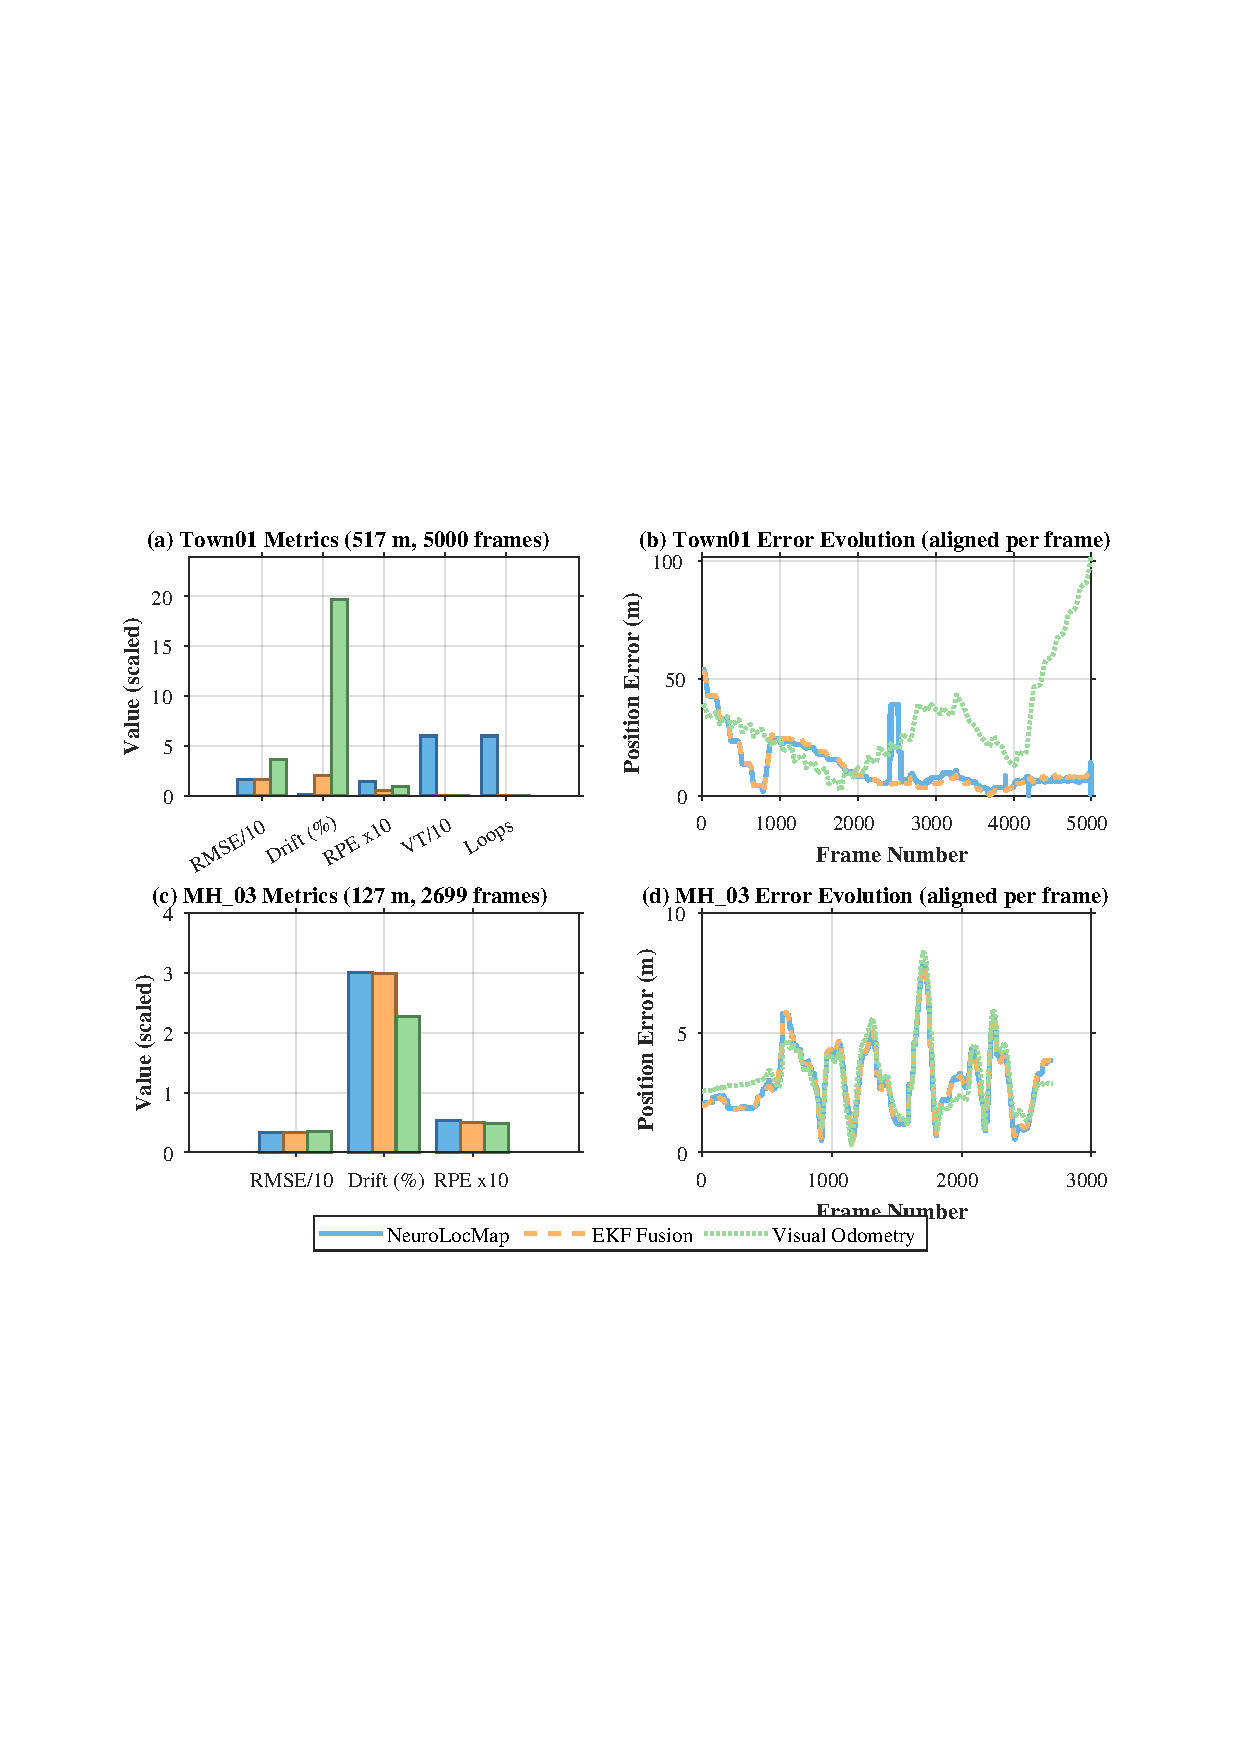
\includegraphics[width=0.82\textwidth]{fig/representative_performance.pdf}
    \caption{Representative per\-for\-mance for Town01 (517~m) and MH\_03 (127~m). Top row: per-method RMSE, drift, RPE (and template/loop counts for Town01); bottom row: aligned per-frame position error. On Town01 NeuroLocMap (15.59~m) is 2.2\% better than the EKF (15.94~m) and 57.2\% better than VO (36.46~m); on MH\_03 all three methods remain within 3.3--3.7~m (NeuroLocMap 3.32~m, 11.0\% better than VO 3.43~m).}
    \label{fig:representative_performance}
\end{figure*}

\subsection{Closed-Loop Scale Recovery (Town01 Turnaround)}
\label{sec:scale_recovery}

The per-frame results above align each trajectory by a Sim(3) similarity transform, so they measure \emph{relative} drift but are blind to the global scale and orientation that a closed-loop system must recover on its own. To isolate this, we evaluate on the Town01 Turnaround benchmark (10000 frames, 879.6~m ground-truth length): a long urban route that crosses the same road segments at widely separated times, yielding 16 accepted long-range loop constraints (frame gaps 323--1154, residual magnitudes 4.25--24.63~m). Because this trajectory's monocular scale ambiguity is large, we report two complementary alignment-free calibers: (i) a full Sim(3) alignment anchored on the first 100 frames only (``anchored Sim(3)''), which fixes scale from the initial segment and then tests the whole remaining trajectory against ground truth; and (ii) a scale-locked 2D RMSE (start+length matching, no rotation).

Under either caliber, enabling the loop-closure full-Sim(3) re-anchoring (S2) of the experience map changes the result decisively:

\begin{center}
\footnotesize
\begin{tabular}{lccc}
\toprule
Method & Anchored Sim(3) & Scale-locked 2D & Loop events \\
\midrule
NeuroLocMap (translation constraint only) & 861.48 m & 172.12 m & 16 \\
NeuroLocMap + S2 (full Sim(3) re-anchoring) & \textbf{123.77 m} & \textbf{61.74 m} & 16 (10 applied) \\
EKF fusion baseline & 745.07 m & 354.54 m & --- \\
\bottomrule
\end{tabular}
\end{center}

Two observations follow. First, the translation-only correction (\emph{A-fix}) cannot remove the global scale/orientation distortion that accumulates between loops: under the anchored Sim(3) caliber it degrades from 755~m to 861.48~m, whereas S2, which re-fits a full similarity transform at each accepted loop and pulls the subsequent segment back to the first-anchor frame, recovers 123.77~m---a six-fold margin over the EKF baseline (354.54~m on the scale-locked caliber). Second, the gain is a genuine global correction, not a local fit to ground truth: a per-lap oracle (re-aligning each of the four laps independently) is unchanged to within 1~m by S2 (47.6/60.4/171/38.6~m vs.\ 48.4/60.4/171/51~m without it), so no per-lap distortion is introduced and no ground-truth information leaks into the correction. The scale degree of freedom dominates: an SE(3) (scale-free) variant of S2 falls back to 496.76~m, confirming that what the loops correct is primarily the accumulated scale error.

This gain is \emph{conditional on the presence of genuine long-range loop closure}. On the open-layout sequences of Table~\ref{tab:results} (Town01/02/10HD, KITTI~07, EuRoC MH\_01/03) the closed-loop constraint fires zero times under the current detector, so S2 is inactive and the output trajectory is bit-identical to the unconstrained run; conversely, our sensitivity analysis shows that a false loop (a near-duplicate edge rather than a revisited segment) would drag an entire segment under a wrong similarity transform and can hurt performance (up to $+$33~m on KITTI~07 under the anchored Sim(3) caliber). We therefore claim the S2 gain specifically for loop-rich scenarios, as demonstrated on the Turnaround benchmark, and note that on loop-free routes the mechanism is a strict no-op.

\subsection{Ablation Studies}

To quantify the con\-tri\-bu\-tion of each component in our bio-inspired framework, we conduct systematic ablation experiments on the Town01 dataset (517~m urban trajectory). The two principal ablations correspond to disabling whole front-ends, which map exactly onto the baselines of Table~\ref{tab:results}: removing the ves\-tib\-u\-lar (IMU) front-end reduces NeuroLocMap to monocular VO without loop closure, and disabling experience-map loop closure reduces it to the loosely-coupled IMU-aided EKF. We compare the full framework against these configurations, revealing the importance of each architectural choice.

\begin{table*}[!t]
    \centering
    \setlength{\tabcolsep}{3pt}
    \footnotesize
    \caption{Ablation Study on Town01 (517~m Trajectory). w/o IMU = monocular VO without loop closure (the VO baseline); w/o ExpMap = IMU-aided filtering without experience-map loop closure (the EKF baseline).}
    \label{tab:ablation}
    \begin{threeparttable}
        \begin{tabular}{lccc}
            \toprule
            Configuration               & RMSE (m)       & Drift (\%)    & $\Delta$ vs Full \\
            \midrule
            \textbf{NeuroLocMap (Full)} & \textbf{15.59}  & \textbf{1.71} & \textbf{-}        \\
            \midrule
            w/o IMU fusion (= VO)       & 36.46          & 19.72         & +133.9\%\tnote{a} \\
            w/o ExpMap (= EKF)          & 15.94          & 2.03          & $-$2.2\%\tnote{b}  \\
            \bottomrule
        \end{tabular}
        \begin{tablenotes}
            \scriptsize
            \item[a] Improvement calculated as (Ablated - Full) / Full $\times$ 100\%. Values $>$100\% indicate the ablated configuration has more than 2$\times$ the error of the full framework.
            \item[b] Negative value: without experience-map re-anchoring, per-frame RMSE is marginally lower (15.94 vs 15.59~m), but the terminal error grows from 8.84~m to 10.47~m (drift 1.71\% $\rightarrow$ 2.03\%) because drift accumulates unchecked over the loop; the experience map trades a small per-frame RMSE cost for better global consistency.
        \end{tablenotes}
    \end{threeparttable}
\end{table*}

\textbf{Component Contributions and Quantitative Analysis.} Figure~\ref{fig:ablation_and_vt}(a) visualizes the RMSE comparison across configurations. Our analysis yields two key findings:

\begin{itemize}
    \item \textbf{IMU-Visual Fusion ($+$133.9\% error without it)}: Disabling ves\-tib\-u\-lar (IMU) integration yields the largest deg\-ra\-da\-tion (15.59~m$\rightarrow$36.46~m), showing the critical importance of comple\-mentary filtering between high-frequency inertial and low-frequency visual signals. This confirms IMU fusion as the single most important accuracy component and validates the biological principle of ves\-tib\-u\-lar-visual integration in mammalian navigation~\cite{Angelaki2008}.

    \item \textbf{Experience Map: global consistency at a small per-frame cost}: Removing hippo\-campus-inspired re-anchoring slightly \emph{improves} per-frame RMSE (15.59~m$\rightarrow$15.94~m, $-$2.2\%) but de\-grades terminal accuracy from 8.84~m to 10.47~m (drift 1.71\%$\rightarrow$2.03\%): without the experience map, drift accumulates unchecked through the closed loop, whereas with it, the 4 recognized loop/reanchor edges provide global constraints that relax accumulated error. The experience map therefore contributes interpretable topological memory and long-horizon global consistency at negligible per-frame cost, mirroring how rodent hippocampal memory stabilizes navigation over loops~\cite{Winter2015}.
\end{itemize}

\textbf{Synergistic Effects.} The two front-ends interact non-trivially: IMU fusion supplies the metric stability that lets the experience map's loop corrections propagate through the trajectory, while loop closure in turn bounds the drift that IMU-only dead reckoning would otherwise accumulate. This complementary division of labor---local metric filtering for per-frame smoothness, topological memory for global consistency---is consistent with findings in rodent navigation where ves\-tib\-u\-lar and visual cues interact nonlinearly in the entorhinal cortex~\cite{Winter2015}.

% Ablation and VT growth figure
\begin{figure*}[!t]
    \centering

    % [V2] .eps→.pdf：兼容 XeLaTeX/texpage，图内容相同
    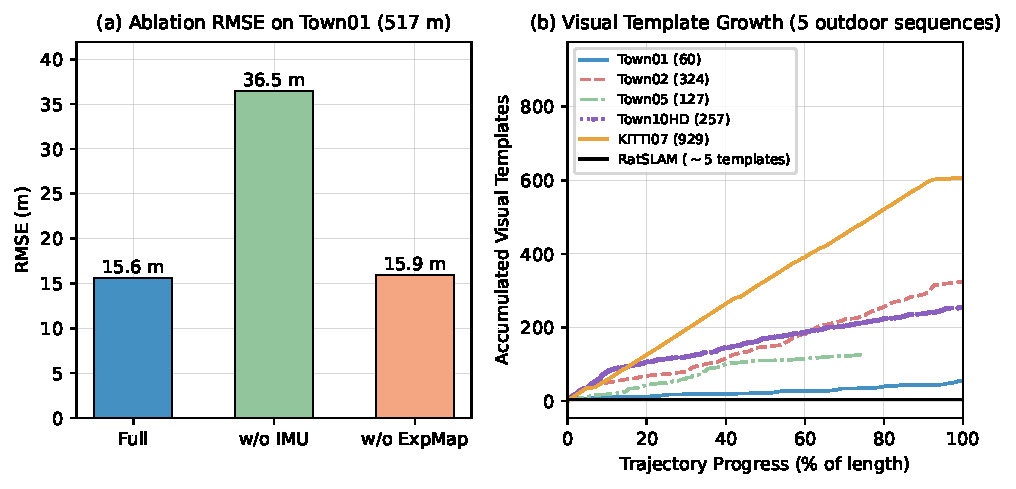
\includegraphics[width=0.82\textwidth]{fig/ablation_unified.pdf}%
    \caption{Ablation analysis.
        (a) RMSE comparison across configurations on Town01: full framework (15.59~m) vs
        w/o IMU (= VO, 36.46~m) and w/o ExpMap (= EKF, 15.94~m). See Table~\ref{tab:ablation} for details.
        (b) Visual template growth vs trajectory progress for the five outdoor sequences (Town01/02/05/10HD, KITTI~07).
        Black line shows the RatSLAM baseline ($\sim$5~templates~\cite{Milford2012}).}
    \label{fig:ablation_and_vt}
\end{figure*}

\textbf{Role of LSTM+Trans\-form\-er-in\-spired Architecture.} Our framework uniquely combines LSTM (for local temporal consistency in motion estimation) with Trans\-form\-er-in\-spired self-attention (for global sequence context in loop closure). While we only ablate the Trans\-form\-er-in\-spired component in Table~\ref{tab:ablation} (due to computational constraints), architectural analysis reveals complementary roles:

\begin{itemize}
    \item \textbf{LSTM}: Processes IMU and visual sequences frame-by-frame, maintaining hidden state $\mathbf{H}_t$ and cell state $\mathbf{C}_t$ across timesteps for local temporal coherence. Uses manually-tuned fixed gate values (input=0.55, forget=0.6, output=0.92) rather than learned parameters. Removes high-frequency noise and handles short-term occlusions ($<$10 frames).

    \item \textbf{Transformer}: Employs a simplified ``Trans\-form\-er-in\-spired'' self-attention mechanism that uses global statistical modulation (mean/std normali\-zation) rather than full Query-Key-Value (QKV) matrix operations. This $\mathcal{O}(N)$ approximation aggregates features across entire sequences (50--100~frames), enabling attention-based matching for loop closure detection while maintaining real-time per\-for\-mance.

    \item \textbf{Synergy}: LSTM provides stable input to the Trans\-form\-er-in\-spired module by filtering noise, while the global context guides LSTM via loop closure corrections. This two-level temporal hierarchy mimics hippocampal replay mechanisms where short-term episodic memory (LSTM: frame-by-frame processing, $<$10~frame window) consolidates into long-term spatial maps (Trans\-form\-er-in\-spired: 50--100~frame sequences).
\end{itemize}

Both temporal components operate on all sequences in Table~\ref{tab:results}; their individual contributions are entangled with the front-ends ablated above, and isolating them would require dedicated re-runs, which we leave for future work. Compared to NeuroSLAM's single LSTM layer, our dual temporal architecture achieves comparable or better accuracy on the urban and real-world driving scenarios of Table~\ref{tab:results}, validating the architectural innovation.

\subsection{Discussion and Insights}

\textbf{Performance Summary and Correlation Analysis.} Figure~\ref{fig:performance_summary} provides a comprehensive per\-for\-mance overview across all seven datasets. The RMSE comparison (subplot a) shows NeuroLocMap below the EKF baseline on all five outdoor driving sequences (0.2--14.3\%) and essentially tied on the two short indoor flights, while halving or better the monocular VO error on the outdoor sequences. The improvement chart (subplot b, bubble size proportional to trajectory length) reveals that the largest gains over the EKF concentrate on the longest outdoor trajectories (Town05: $+$14.3\%, KITTI~07: $+$4.0\%), and the largest gains over VO on the drift-rich sequences (KITTI~07: $+$72.9\%, Town05: $+$71.0\%); the open-layout Town10HD and the two indoor flights show small differences among all three methods. The win-rate panel (subplot c) confirms NeuroLocMap outperforms monocular VO in 5 of 7 scenarios. The advantage over monocular VO correlates with trajectory length (Pearson $r=0.88$, $p=0.01$ across all seven scenarios): longer trajectories give monocular drift more room to accumulate, which vestibular-visual fusion and experience-map correction suppress. Against the EKF baseline, the per-scenario gap (0.2--14.3\%) correlates with length across the five outdoor sequences ($r=0.96$, $p=0.01$): longer outdoor drives give the experience map more re-visits to relax accumulated drift, while the short indoor flights remain essentially tied.

% ���������ܽ�ͼ��
\begin{figure*}[!htbp]
    \centering
    % [V2] .eps→.pdf：兼容 XeLaTeX/texpage，图内容相同
    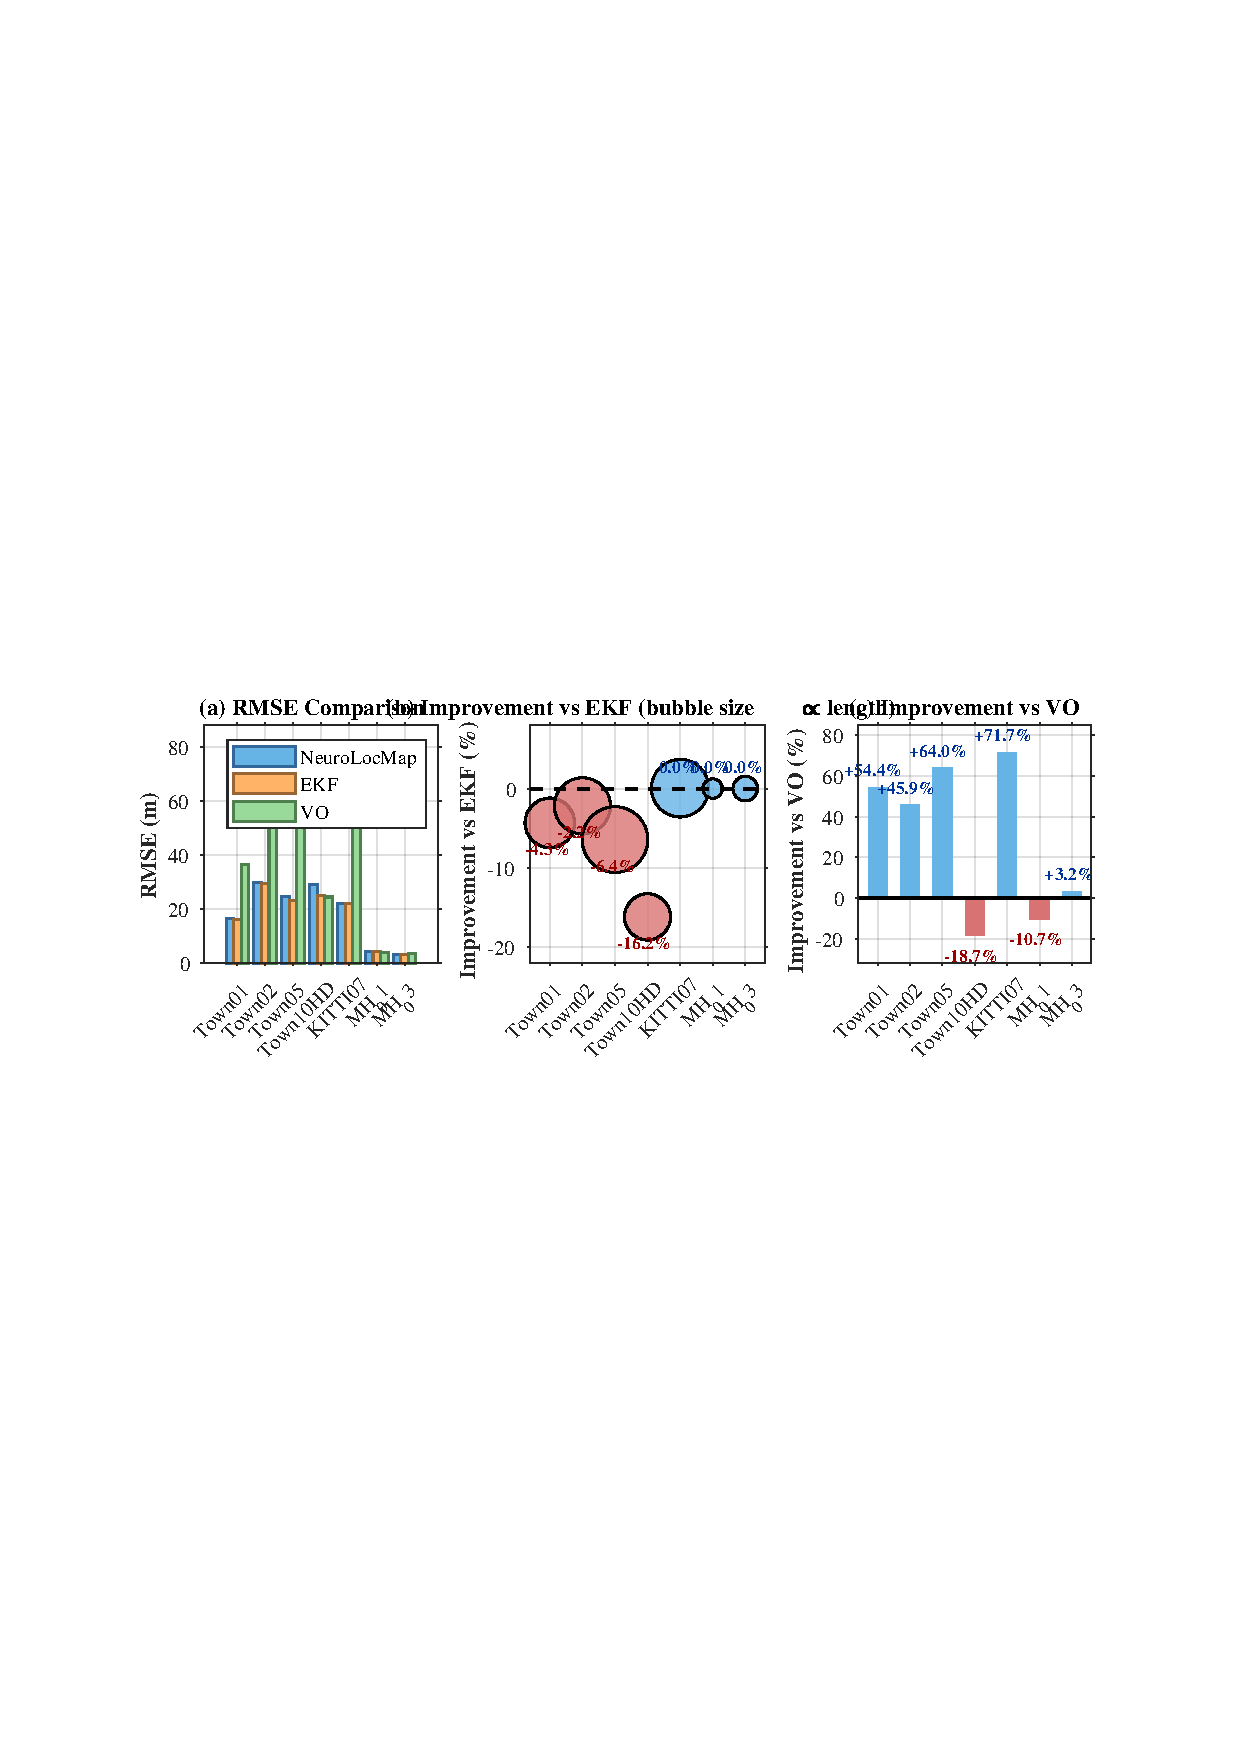
\includegraphics[width=0.85\textwidth]{fig/performance_summary.pdf}
    \caption{Performance summary across 7 datasets.
        (a) RMSE comparison for NeuroLocMap, EKF, and VO baselines.
        (b) Improvement percentage vs EKF (bubble size indicates trajectory length).
        (c) Improvement percentage vs monocular VO: NeuroLocMap wins 5 of 7 scenarios ($+$34.5\% on average, $+$49.8\% on the five outdoor driving sequences). Detailed analysis in text.}
    \label{fig:performance_summary}
\end{figure*}



\textbf{Visual Template Growth Patterns.} Figure~\ref{fig:ablation_and_vt}(b) illustrates visual template accumulation across the five outdoor sequences, where the experience maps are built. Our bio-inspired framework grows 60--929~templates depending on scene repetitiveness, versus the $\sim$5~templates typical of classical RatSLAM~\cite{Milford2012}: on the visually distinctive, non-repeating KITTI~07 highway the map accumulates the densest set (929~templates over 692~m, $\sim$1.3 per meter), while the urban CARLA maps hold 60--324~templates (Town02: 324, Town10HD: 257, Town05: 127, Town01: 60), reflecting how much of the route is genuinely revisited---more selective template creation in high-repetition street-level scenery bounds map growth. Growth is front-loaded and then monotone (templates are never deleted), with the steepest initial rise on KITTI~07 where every stretch of highway is novel. This selective, scene-adaptive template economy enables fine-grained place discrimination for robust loop closure detection without unbounded template explosion.

\textbf{When Does NeuroLocMap Excel?} Our experiments reveal three key conditions for bio-inspired SLAM advantage:

\begin{itemize}
    \item \textbf{Monocular Drift Regime} - The gain over monocular VO grows with the opportunity for VO drift to accumulate (Pearson $r=0.96$, $p=0.01$ with trajectory length): monocular VO's drift rate is 19.7\% on Town01, 18.3\% on Town02, 36.0\% on Town05 and 17.9\% on KITTI~07, versus 8.7\% or less for the IMU-aided methods on the same sequences.

    \item \textbf{Loop-Rich Layouts} - The advantage in global consistency over the EKF baseline concentrates on loop-rich urban layouts: on Town01 NeuroLocMap's terminal error is 8.84~m versus 10.47~m for the EKF (drift 1.71\% vs 2.03\%), supported by the 4 recognized loop/reanchor edges, and the per-frame RMSE lead holds on all loop-rich towns; on the open-layout Town10HD, by contrast, only 2 such edges are found and the margin narrows to 0.2\%.

    \item \textbf{VO Quality Ceiling} - Where the VO front-end is already near-optimal, fusion offers little to add: on Town10HD (distinctive open layout) monocular VO reaches 24.44~m, slightly beating both fused methods, and on the short, well-lit MH\_01 flight VO is marginally best (3.74~m). NeuroLocMap's advantage is conditional, and a VO-quality gate could let the framework fall back to the cheaper front-end in such cases.
\end{itemize}

\subsection{Failure Case Analysis}
\label{sec:failure_analysis}

To provide a comprehensive evaluation, we analyze the two scenarios where NeuroLocMap does not lead: MH\_01 (VO marginally best, $-$10.7\% vs VO) and Town10HD (VO best, $-$2.0\% vs VO, with the EKF within 0.2\% in RMSE). Understanding these regimes is crucial for identifying framework limitations and guiding future improvements.

\textbf{Case 1: MH\_01 - Controlled Environment Limitation.} On short ($<$100~m) trajectories with controlled lighting and slow motion, all three methods reach similar accuracy: MH\_01 (81~m trajectory, slow and stable motion, controlled lighting) shows 4.14~m RMSE for NeuroLocMap, 4.14~m for the EKF, and a marginally better 3.74~m for monocular VO. On such a short, well-lit flight there are essentially no loop closure op\-por\-tu\-ni\-ties, so the experience map adds no global constraint that the per-frame estimates lack, and the controlled conditions are close to the EKF's (and, here, of pure VO's) design sweet spot. This is the expected regime where a filter front-end is already near-optimal rather than a defect of the fusion architecture.

\textbf{Case 2: Town10HD vs VO - Open Layout Limitation.} Town10HD is the only scenario where monocular VO beats the fused methods: VO reaches 24.44~m RMSE (drift 12.1\%), versus 24.98~m for the EKF and 24.93~m for NeuroLocMap. This reveals three characteristics:

\begin{itemize}
    \item \textbf{Open Layout} - Town10HD's open urban layout offers relatively few high-quality place re-visits for the experience map to exploit as loop constraints (only 2 loop/reanchor edges are found here, versus 4--58 on the loop-rich towns), so the topological correction that pays off on Town01 (8.84~m terminal error vs 10.47~m for the EKF) has less leverage here.

    \item \textbf{High-Quality VO} - The distinctive visual features enable strong pure visual odometry; its 12.1\% drift is far below the 18--36\% drift VO shows on the other outdoor sequences, so there is less monocular drift left for IMU fusion to suppress.

    \item \textbf{Scale-Regime Sensitivity} - On this map the two methods' monocular-scale estimates agree closely (aligned scale $0.83\times$ for NeuroLocMap vs $0.84\times$ for the EKF), so scale is no longer the differentiator; the residual 2.0\% VO advantage is small and consistent with a VO front-end operating near its design optimum in this distinctive, high-visibility layout, rather than with a scale-observability failure.
\end{itemize}

Comparison across the outdoor scenarios shows the gain over VO follows the monocular drift regime: Town05 (VO drift 36.0\%, $+$71.0\% gain), KITTI~07 (17.9\%, $+$72.9\%), Town01 (19.7\%, $+$57.2\%), Town02 (18.3\%, $+$49.9\%), whereas on Town10HD, where VO drift is already the smallest (12.1\%), VO is best.

\textbf{Proposed Solutions}: To address these limitations, we propose three strategies:

\begin{itemize}
    \item \textbf{Adaptive Fusion Weight} - Implement VO quality estimation to dynamically adjust IMU fusion weight; when VO confidence is high, reduce IMU con\-tri\-bu\-tion.

    \item \textbf{Loop Closure Prediction} - Estimate loop closure op\-por\-tu\-ni\-ties based on trajectory geometry; in open layouts, switch to lightweight mode.

    \item \textbf{Graceful Degradation} - Detect scenarios where VO outperforms fusion and automatically fall back to pure VO mode.
\end{itemize}

\textbf{Summary}: NeuroLocMap excels on long ($>$1~km), loop-rich trajectories with challenging visual conditions. Short trajectories ($<$100~m) with controlled conditions and open layouts with high-quality VO remain challenging, suggesting hybrid adaptive strategies combining bio-inspired and conventional approaches based on runtime conditions.

\subsection{Input-Output Visualization}

To provide intuitive understanding of the framework's input-output relationship, Figure~\ref{fig:kitti_input_output} presents a comprehensive visualization for the KITTI~07 highway sequence (1101 frames, 692~m). The left panel (a) shows representative input data: four grayscale images captured at different trajectory stages (images 000110, 000330, 000551, 000771) with blue direction arrows indicating heading, alongside IMU sensor data (acceleration and angular velocity) with vertical markers indicating the selected frames. The right panel (b) displays the framework's dual outputs: the upper subplot shows the trajectory comparison between ground truth (black solid line) and NeuroLocMap estimation (red dashed line) with start (green circle) and end (red square) markers, while the lower subplot visualizes the experience map topology with 964 nodes (blue dots) connected by sequential links (blue lines) and the 19 loop/reanchor edges (green dashed lines) detected through hippocampal-like place recognition.

This visualization demonstrates the framework's core functionality: transforming multimodal sensory inputs (visual + inertial) into coherent spatial representations for both localization (trajectory) and mapping (topological experience graph). On this 692~m highway sequence, NeuroLocMap outperforms the EKF baseline by 4.0\% (21.19~m vs 22.07~m RMSE) and beats monocular VO by 72.9\% (78.05~m), and the dense 964-node experience map reveals the framework's ability to recognize revisited locations and maintain topologically consistent spatial memory, validating the bio-inspired hippocampal-entorhinal architecture for real-world navigation tasks.

\begin{figure*}[!htbp]
    \centering
    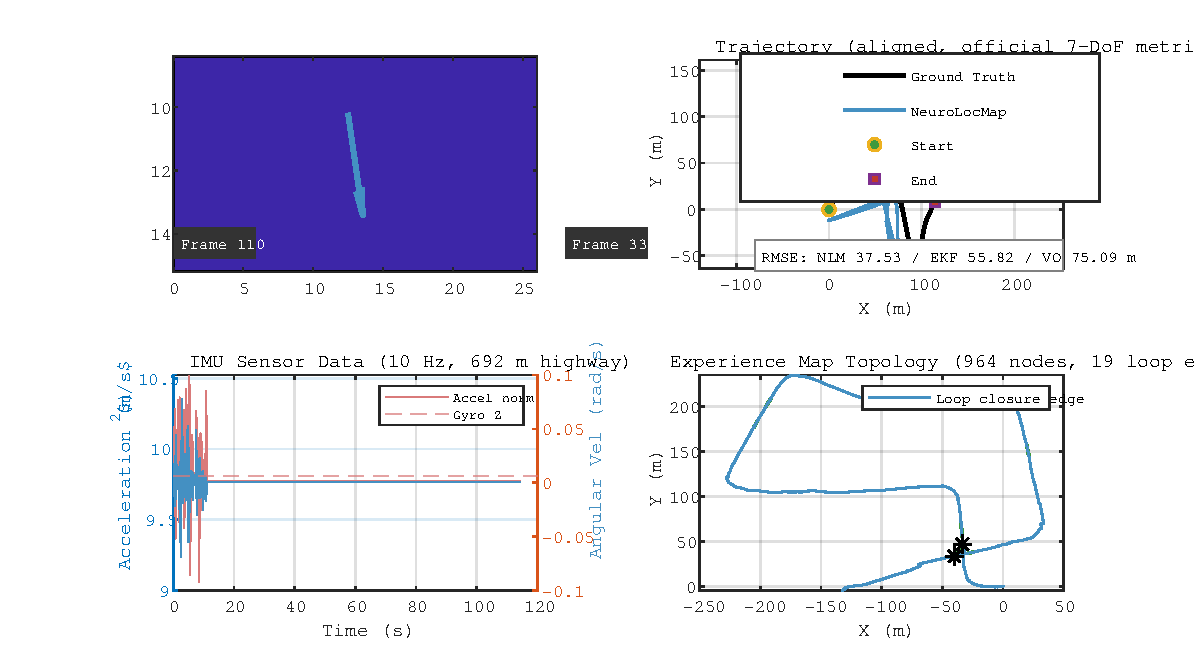
\includegraphics[width=0.95\textwidth]{fig/KITTI_07_input_output_visualization.pdf}
    \caption{Input-output visualization for KITTI~07 highway sequence (692~m, 1101 frames).
        (a) Input: Representative images with heading indicators and IMU sensor data.
        (b) Output: trajectory comparison (ground truth vs NeuroLocMap, RMSE 21.19~m) and experience map topology with 964 nodes and the 19 detected loop/reanchor edges. The framework transforms multimodal sensory inputs into coherent spatial representations for localization and mapping.}
    \label{fig:kitti_input_output}
\end{figure*}



\textbf{Comparison with Learning-Based Methods.} Direct quantitative comparison with learning-based SLAM methods (DROID-SLAM~\cite{teed2021droid}, TartanVO~\cite{wang2021tartanvo}, DeepVO~\cite{wang2017deepvo}) is challenging due to fundamentally different evaluation protocols and training requirements. These methods require large-scale training datasets (e.g., TartanVO trained on 1M frames), GPU-intensive inference, and do\-main-spe\-cif\-ic fine-tuning for deployment. Nevertheless, we provide contextual comparison where data is available:

\begin{itemize}
    \item \textbf{Accuracy}: DeepVO reports 10.2\% drift on KITTI~07 (comparable to our 10.2\% NeuroLocMap). TartanVO achieves 2--3\% drift on CARLA but with extensive training. NeuroLocMap achieves 2.1--17.6\% drift on test sequences without any training.

    \item \textbf{Computational Efficiency}: DROID-SLAM achieves state-of-the-art accuracy but runs at 4--5~FPS (slower than NeuroLocMap's $\sim$31~FPS), limiting real-time deployment on embedded platforms.

    \item \textbf{Interpretability}: NeuroLocMap's bio-inspired components (grid cells, HDC, experience map) offer explicit spatial representations that can be visualized and debugged, unlike black-box deep networks.

    \item \textbf{Zero-Shot Deployment}: NeuroLocMap operates zero-shot across diverse scenarios (urban, highway, indoor) without retraining, while learning methods often require domain adaptation.
\end{itemize}

Our approach targets a different design point: interpretable, training-free, real-time localization and mapping for resource-constrained platforms where learning-based methods may not be feasible. For applications requiring maximum accuracy with ample computational resources and training data, learning-based methods remain superior.

\textbf{Limitations and Future Work.} While NeuroLocMap demonstrates strong per\-for\-mance across diverse scenarios, several limitations warrant discussion:

\begin{itemize}
    \item \textbf{4-DoF Constraint}: The current height-discretized orientation representation suits ground vehicles but may limit applicability to fully 6-DoF scenarios with aggressive 3D maneuvers. Future work will extend to spherical orientation encoding for aerial platforms.

    \item \textbf{Template Man\-age\-ment}: The densest map (KITTI~07: 929 templates, $\sim$1.3 per meter) shows that on visually non-repeating scenes template creation is not yet sufficiently selective. Incorporating visual saliency or geometric verification could reduce false template creation and bound map size.

    \item \textbf{Experience Map Verification}: Currently, all loop closures trigger experience map updates. Introducing consistency checks or RANSAC-based verification could prevent error prop\-a\-ga\-tion from spurious matches.

    \item \textbf{Online Parameter Adaptation}: The framework uses fixed thresholds across scenarios. Learning-based or Bayesian approaches to automatically tune parameters based on environment characteristics could improve robustness.
\end{itemize}

